\chapter{페르미온 질량: 카이랄성, 유카와 결합, 마요라나 중성미자}

\lectureoverview{먼저 장난감 \(U(1)\) 이론에서 게이지 보손의 힉스 메커니즘을 다시 살펴본 뒤, 페르미온에 대해서도 이에 대응하는 질문을 던진다. 디랙 질량은 왼쪽 카이랄 장과 오른쪽 카이랄 장을 섞지만, 약한 상호작용은 이들에 서로 다른 전하를 부여하므로 맨 질량항을 허용하지 않는다. 힉스 장과의 유카와 결합은 대칭성을 보존한다. 힉스 장이 진공 기댓값을 얻으면 같은 상호작용이 페르미온 질량이 되고, 측정 가능한 힉스--페르미온 결합으로 나타난다. 마지막 부분에서는 이 논리를 따라 중성미자 질량, 보호받지 못하는 무거운 입자의 가능성, 우주선의 운동학, 상대론적 관성, 중력을 살펴본다.}

도입부의 복습은 앞선 강의를 그저 되풀이하기 위한 것이 아니다. 그 내용에서 페르미온에도 적용할 수 있는 개념 하나를 가져와야 한다. 질량은 운동량이 영인 들뜸에 대응하는 영이 아닌 에너지다. 장에서 운동량이 영이라는 것은 파장이 무한대이거나 변위가 모든 곳에서 같다는 뜻이다. 미분항만 있는 이론은 균일한 변위를 감지할 수 없다. 미분항이 없는 항은 감지할 수 있다.

\section{한 번에 살펴보는 게이지 보손 이야기}

\subsection{미분 에너지와 질량 없는 벡터장}

모형 게이지 장은 \(A_\mu\)이고, 장세기는 다음과 같다.
\begin{equation}
  F_{\mu\nu}
  =\partial_\mu A_\nu-\partial_\nu A_\mu .
  \label{eq:l09-field-strength}
\end{equation}
판서에서는 게이지 운동항을 개략적으로 \(F^2\)라고 쓴다. 표준적인 정규화를 적용하면 다음과 같다.
\begin{equation}
  \mathcal L_{\mathrm{gauge}}
  =-\frac14 F_{\mu\nu}F^{\mu\nu}.
  \label{eq:l09-gauge-kinetic}
\end{equation}

\begin{figure}[htbp]
\centering
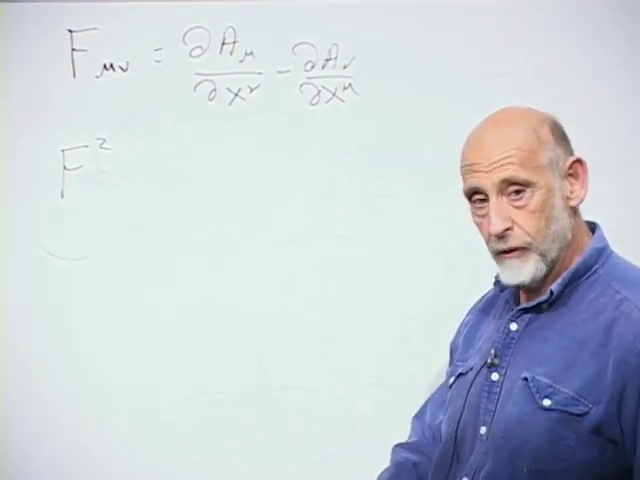
\includegraphics[width=0.72\textwidth]{lecture_09_figure_02.png}
\caption{게이지 장의 장세기 정의와 게이지 장의 미분 에너지를 나타내는 판서의 \(F^2\) 약식 표기.}
\lectureframe{00:02:39}
\label{fig:l09-field-strength-board}
\end{figure}

\(A_\mu\)는 \eqref{eq:l09-gauge-kinetic}에서 나타날 때마다 미분된다. 따라서
\begin{equation}
  A_\mu(x)\longmapsto A_\mu(x)+c_\mu,
  \qquad \partial_\nu c_\mu=0,
\end{equation}
는 \(F_{\mu\nu}\)를 바꾸지 않는다. 그러므로 균일한 벡터 퍼텐셜에는 장세기 에너지가 들지 않는다. 강의의 표현을 빌리면, 운동량이 0인 모드에는 갭이 없고 게이지 보손은 질량이 없다.

이 \(U(1)\) 장은 의도적으로 단순화한 대용물이다. 실제 대상은 전자기 광자가 아니라 \(W^\pm\)와 \(Z\)이다. 깨지지 않은 전자기 대칭성은 광자를 질량 없는 상태로 두지만, 깨진 전약 대칭성은 약한 게이지 보손에 질량을 부여한다.

\subsection{힉스장의 반지름을 고정하기}

전하를 띤 복소 스칼라장을 도입하고 극형식으로 쓰면,
\begin{equation}
  \phi(x)=\rho(x)e^{i\alpha(x)}.
\end{equation}
멕시코 모자형 퍼텐셜은 반지름이 영이 아닌 원 위에서 최소가 된다. 그 반지름을 \(f\)라 하자. 반지름 방향은 비교적 강직하다. 우선 반지름은 고정하고 위상만 남겨 두자.
\begin{equation}
  \phi(x)\simeq f e^{i\alpha(x)}.
  \label{eq:l09-frozen-higgs}
\end{equation}

\begin{figure}[htbp]
\centering
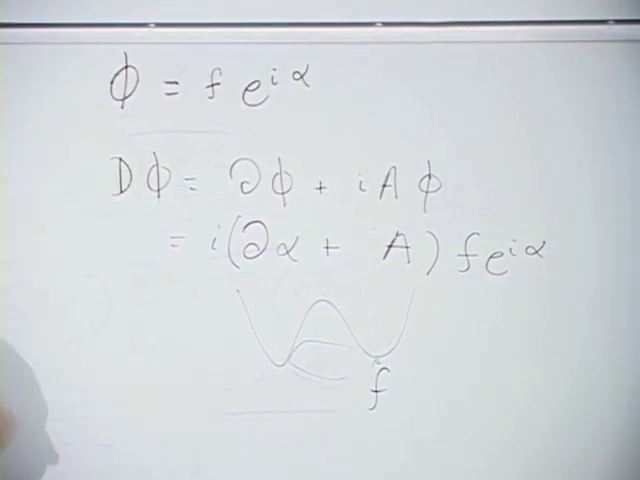
\includegraphics[width=0.72\textwidth]{lecture_09_figure_03.png}
\caption{고정된 힉스 반지름과 그 공변미분, 그리고 복습에서 사용한 깨진 퍼텐셜의 간략한 그림.}
\lectureframe{00:06:42}
\label{fig:l09-frozen-board}
\end{figure}

다음 규약을 택하자.
\begin{equation}
\begin{aligned}
  D_\mu&=\partial_\mu+igA_\mu,
  \\
  \phi&\longmapsto e^{i\theta}\phi,
  \\
  A_\mu&\longmapsto A_\mu-\frac1g\partial_\mu\theta .
\end{aligned}
  \label{eq:l09-gauge-convention}
\end{equation}
강의에서는 \(g\)를 생략하지만, 이를 드러내 두면 차원과 최종 질량을 분명히 알 수 있다. 고정된 장에 작용시키면
\begin{align}
  D_\mu\phi
  &=(\partial_\mu+igA_\mu)f e^{i\alpha}
  \notag\\
  &=i\bigl(\partial_\mu\alpha+gA_\mu\bigr)
    f e^{i\alpha}.
  \label{eq:l09-covariant-frozen}
\end{align}
복소켤레를 곱하면 위상이 사라지고, \(i\)와 \(-i\)의 곱도 \(+1\)이 된다.
\begin{equation}
  |D_\mu\phi|^2
  =f^2
   \bigl(\partial_\mu\alpha+gA_\mu\bigr)
   \bigl(\partial^\mu\alpha+gA^\mu\bigr).
  \label{eq:l09-frozen-square}
\end{equation}

\begin{classroomqa}\audiencequestion{미분에서 \(i\)가 나오므로 공변미분의 제곱에는 음의 부호가 붙어야 하나요?
\lecturetimestamp{00:07:39}}\lecturerresponse{아니다. 운동항은 복소켤레와 곱한 것이다. 한 인자에서는 \(i\)가, 다른 인자에서는 \(-i\)가 나오므로 \(i(-i)=1\)이다. \(D_\mu\)의 부호 규약은 일관되게 뒤집을 수 있지만, 이에 대응하는 에너지 식에서 절댓값의 제곱은 양수다.}\end{classroomqa}

\eqref{eq:l09-frozen-square}의 조합 자체가 이동된 게이지 장이다. \(\theta=-\alpha\)를 택해 스칼라 위상을 없애고, 다음과 같이 정의하자.
\begin{equation}
  A'_\mu=A_\mu+\frac1g\partial_\mu\alpha .
  \label{eq:l09-unitary-gauge-field}
\end{equation}
그러면
\begin{equation}
  |D_\mu\phi|^2=g^2f^2 A'_\mu A'^\mu .
  \label{eq:l09-vector-mass-term}
\end{equation}
새 항에는 \(A'_\mu\)의 미분이 없다. 이제 균일한 장에도 에너지가 저장되므로, 운동량이 0인 벡터 모드에는 갭이 생긴다.

\begin{figure}[htbp]
\centering
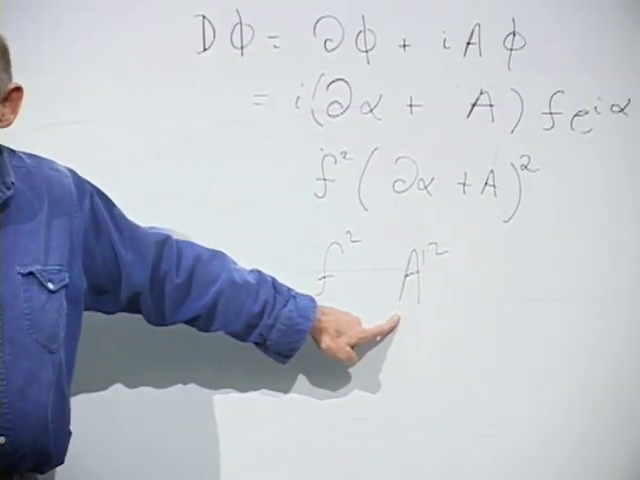
\includegraphics[width=0.72\textwidth]{lecture_09_figure_04.png}
\caption{위상을 흡수한 뒤 게이지 보손 질량이 생겼음을 나타내는 \(f^2A^2\) 항을 판서에서 따로 보여준다.}
\lectureframe{00:10:31}
\label{fig:l09-vector-mass-board}
\end{figure}

스칼라장을 표준적으로 정규화하면
\(\phi=(f+h)e^{i\pi/f}/\sqrt2\)로 쓴다. 이를 벡터 항 \(\tfrac12m_A^2A_\mu A^\mu\)와 비교하면 이 아벨 모형에서
\begin{equation}
  m_A=gf
  \label{eq:l09-abelian-vector-mass}
\end{equation}
을 얻는다. 강의에서는 정규화 인자를 생략하고 벡터 질량이 \(f\)로 정해진다고 요약한다.

위상 모드가 아무런 설명 없이 사라진 것은 아니다. 게이지화하기 전에는 질량 없는 골드스톤 보손이었다. 게이지화한 뒤에는 질량 있는 벡터 입자에 필요한 종방향 편광을 제공한다. 잠시 고정해 두었던 반지름 방향 요동은 물리적인 힉스 들뜸으로 남는다.

\subsection{미분이 없는 항은 왜 질량을 뜻하는가}

\begin{classroomqa}\audiencequestion{\(A'^2\) 항은 왜 단순히 또 다른 상호작용이 아니라 질량으로 간주되나요?
\lecturetimestamp{00:13:10}}\lecturerresponse{질량은 정지 상태의 에너지다. 장에서 정지한 입자는 운동량이 0이고 파장이 무한대인 모드의 양자다. 미분항은 정적으로 균일한 변위에 에너지를 주지 않지만, \(m_A^2A'^2\)는 에너지를 준다. 운동량이 0일 때 생기는 이 비영 에너지가 정지 에너지 갭이다.}\end{classroomqa}

강의에서는 이 내용을 세 가지 역학적 비유로 설명한다.

\begin{itemize}
  \item 결정에서는 이웃한 원자들이 서로 다르게 이동하므로, 변위가 위치에 따라 천천히 변해도 탄성 에너지가 든다. 모든 원자를 함께 옮기는 강체 병진에는 내부 에너지가 들지 않는다. 따라서 음향 포논은 갭이 없다.
  \item 이상적으로 회전 대칭인 자석에서는 스핀 방향이 공간에 따라 변하면 교환 에너지가 들지만, 모든 스핀을 함께 회전시키는 데는 에너지가 들지 않는다. 이에 대응하는 장파장 스핀파는 갭이 없다.
  \item 플라스마에서 전자 유체를 양전하 배경에 대해 이동시키면, 상대 변위가 균일하더라도 전하 분리가 생기고 복원 전기장이 형성된다. 그 결과 플라스몬은 파수가 영일 때도 영이 아닌 진동수를 갖는다.
\end{itemize}

힉스 메커니즘으로 질량을 얻은 게이지 장은 세 번째 사례와 같이 거동한다. 깨진 매질은 그렇지 않았다면 에너지가 들지 않았을 균일한 변위에 저항한다.

\begin{classroomqa}\audiencequestion{게이지 장을 도입하기 전에도 위상 \(\alpha\)는 이미 진동하지 않았나요?
\lecturetimestamp{00:18:24}}\lecturerresponse{진동했다. 그 에너지는 \(f^2(\partial_\mu\alpha)^2\)에 비례했다. 위치마다 달라지는 위상에는 기울기 에너지가 있어 전파될 수 있지만, 균일한 위상 변화에는 에너지가 들지 않는다. 이것이 바로 질량 없는 골드스톤 모드다.}\end{classroomqa}

\begin{classroomqa}
\audiencequestion{미분에는 시간 미분도 포함됩니다. 격자 전체를 실제로 움직이거나 장 전체를 변화시키면 운동 에너지가 생기지 않나요?\lecturetimestamp{00:22:18}}
\lecturerresponse{그렇습니다. 여기서 비교하는 것은 정적인 배치들이거나 원하는 만큼 천천히 준비한 배치들입니다. 격자가 영이 아닌 속도로 병진하면 운동 에너지가 있습니다. 질량을 판별할 때 묻는 것은 배치가 정지해 있고 공간적으로 균일해도 에너지가 남는가 하는 점입니다.}
\end{classroomqa}

\section{실험적 단서: 약한 상호작용은 왼쪽과 오른쪽을 구별한다}

이제 강의는 전자, 뮤온, 쿼크를 살펴본다. 이들의 질량도 힉스 장에서 비롯되지만, 페르미온 질량은 이차 벡터 항이 아니므로 메커니즘의 형태가 다르다. 페르미온 질량은 두 카이랄 장 사이의 결합이다.

\subsection{베타 붕괴에서의 패리티 위반}

먼저 약한 상호작용이 패리티를 위반한다는 실험적 사실에서 출발하자. 양자전기역학과 양자색역학에서는 어떤 과정과 그 거울상이 똑같이 다뤄진다. 약한 상호작용은 그렇지 않다. 중성자 베타 붕괴에서는
\begin{equation}
  n\longrightarrow p+e^-+\bar\nu_e,
  \label{eq:l09-beta-decay}
\end{equation}
전하 전류 상호작용이 선택하는 고에너지 전자의 헬리시티가 왼손잡이다. 즉 스핀은 운동량과 반대 방향을 향한다. 이에 대응하는 반중성미자의 헬리시티는 반대다.

초상대론적 입자의 헬리시티를 다음과 같이 정의하자.
\begin{equation}
  h=\frac{\bm S\cdot\bm p}{|\bm S|\,|\bm p|}.
\end{equation}
스핀과 운동량이 나란하면 \(h=+1\)이고, 서로 반대 방향이면 \(h=-1\)이다. 약한 상호작용은 왼쪽 카이랄 전자 장과 왼쪽 카이랄 중성미자 장에 결합하며, 오른쪽 카이랄 전자 장에는 같은 방식으로 결합하지 않는다.\editorialnote{강의에서는 고에너지에서 시각적으로 직관적이라는 이유로 처음에 헬리시티의 의미로 손잡이성을 사용한다. 그러나 게이지 전하는 카이랄성, 즉 \(P_L=(1-\gamma^5)/2\)와 \(P_R=(1+\gamma^5)/2\)가 선택하는 로런츠 표현의 표지에 작용한다. 질량 없는 입자에서는 입자의 카이랄성과 헬리시티가 일치하지만, 질량 있는 입자에서는 그렇지 않다.}

전체 \(SU(2)_L\times U(1)_Y\) 장부를 다루지 않고도 장애물을 드러내기 위해, 관련 전하를 \(\psi_L\)만 갖는 가상의 \(U(1)\) 세계를 생각해 보자.
\begin{equation}
  \psi_L\longmapsto e^{i\theta}\psi_L,
  \qquad
  \psi_R\longmapsto\psi_R .
  \label{eq:l09-chiral-toy-charge}
\end{equation}
이는 전자기 이론이 아니다. 실제로 왼쪽과 오른쪽 카이랄 전자는 같은 전기 전하를 갖는다. 이는 두 카이랄성이 서로 다른 전약 표현에 속하는 약한 상호작용을 단순화해 그린 것이다.

\begin{classroomqa}\audiencequestion{쿼크에도 같은 왼쪽--오른쪽 비대칭이 적용되나요?
\lecturetimestamp{00:31:50}}\lecturerresponse{그렇다. 단, 알맞은 약한 다중항과 초전하를 고려해야 한다. 왼쪽 카이랄 업형 및 다운형 쿼크는 약한 이중항을 이루지만, 오른쪽 카이랄 장은 약한 단일항이다. 따라서 쿼크의 힉스 결합에도 전자의 경우와 같은 구조적 문제가 생긴다.}\end{classroomqa}

\section{디랙 질량은 왼쪽--오른쪽 혼합이다}

\subsection{4성분 방정식에서 두 바일 방정식으로}

디랙 파동함수는 네 성분을 갖는다. 대략 말해 두 성분은 스핀을 나타내고, 나머지 두 성분은 양에너지 해와 음에너지 해를 구별하며, 음에너지 해는 반입자 자유도로 다시 해석된다. 해밀토니안 형식으로 쓰면
\begin{equation}
  i\frac{\partial\Psi}{\partial t}
  =\left(-i\bm\alpha\cdot\bm\nabla+m\beta\right)\Psi .
  \label{eq:l09-dirac-hamiltonian}
\end{equation}
행렬 \(\alpha_i\)와 \(\beta\)는 에너지, 운동량, 질량 사이의 상대론적 관계를 나타낸다.

\begin{figure}[htbp]
\centering
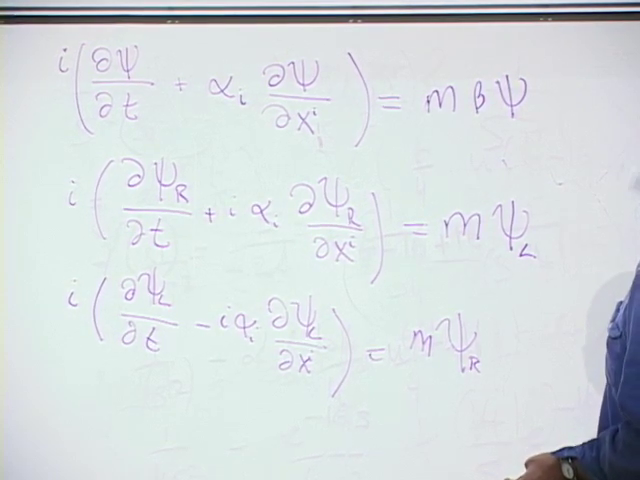
\includegraphics[width=0.74\textwidth]{lecture_09_figure_05.png}
\caption{판서에서는 먼저 디랙 방정식을 쓴 다음, 이를 결합된 왼쪽 및 오른쪽 손잡이 방정식으로 나눈다.}
\lectureframe{00:40:30}
\label{fig:l09-dirac-board}
\end{figure}

카이랄 기저를 쓰면 \(m\)의 역할이 명확해진다. \(\sigma^\mu=(1,\bm\sigma)\)와 \(\bar\sigma^\mu=(1,-\bm\sigma)\)를 두면
\begin{align}
  i\bar\sigma^\mu\partial_\mu\psi_L&=m\psi_R,
  \label{eq:l09-weyl-left}\\
  i\sigma^\mu\partial_\mu\psi_R&=m\psi_L.
  \label{eq:l09-weyl-right}
\end{align}
\(m=0\)일 때 두 방정식은 서로 독립이다. 왼쪽 카이랄 장과 오른쪽 카이랄 장은 서로 영향을 주지 않고 전파될 수 있다. \(m\neq0\)일 때는 각 장이 다른 장의 원천으로 나타난다. 이것이 디랙 질량이 왼쪽과 오른쪽을 섞는다는 말의 정확한 의미다.

Susskind는 이를 페르미온이 왼쪽과 오른쪽 사이에서 진동한다고 설명한다. 이 표현은 결합을 잘 나타내지만, 점입자가 고전적으로 앞뒤로 뒤집힌다는 뜻으로 받아들여서는 안 된다. 정확한 진술은 결합된 장 방정식 \eqref{eq:l09-weyl-left}--\eqref{eq:l09-weyl-right}이다.

\begin{classroomqa}\audiencequestion{판서에 나온 두 방정식의 \(i\) 인자와 부호는 서로 일관되나요?
\lecturetimestamp{00:41:10}}\lecturerresponse{판서의 줄마다 일관되지는 않는다. 빠르게 유도하는 과정에서 \(i\) 하나를 일관성 없이 바깥으로 뺐다. 신뢰할 수 있는 내용은 결합 구조다. 방정식 \eqref{eq:l09-weyl-left}과 \eqref{eq:l09-weyl-right}은 표준적인 일관된 규약 하나를 제시한다.}\end{classroomqa}

\subsection{약한 대칭성은 왜 맨 질량항을 금지하는가}

이에 대응하는 디랙 질량항은 라그랑지안에서
\begin{equation}
  \mathcal L_m
  =-m\bar\psi\psi
  =-m\left(\bar\psi_L\psi_R+\bar\psi_R\psi_L\right).
  \label{eq:l09-bare-dirac-mass}
\end{equation}
이다. 장난감 변환 \eqref{eq:l09-chiral-toy-charge} 아래에서
\begin{equation}
  \bar\psi_L\psi_R\longmapsto
  e^{-i\theta}\bar\psi_L\psi_R,
  \qquad
  \bar\psi_R\psi_L\longmapsto
  e^{i\theta}\bar\psi_R\psi_L.
\end{equation}
두 항 중 어느 것도 불변이 아니다. 따라서 대칭성이 깨지기 전에는 직접적인 왼쪽--오른쪽 혼합 계수 \(m\)가 금지된다.

전자기 상호작용만으로는 이 문제가 생기지 않는다. \(\psi_L\)와 \(\psi_R\)의 전기 전하가 같기 때문이다. 장애물은 이들의 약한 양자수가 서로 다르다는 데서 생긴다.

\subsection{카이랄성의 미묘함을 드러내는 헬리시티 질문}

이제 수업에서는 직관적인 손잡이성 그림을 여러 각도에서 살펴본다. 이 질문들은 부수적인 문제가 아니다. 헬리시티가 유용한 경우와 카이랄성으로 대신해야 하는 경우를 정확히 드러낸다.

\begin{classroomqa}\audiencequestion{약한 상호작용이 두 헬리시티의 전자를 똑같은 비율로 방출한다면 세계는 어떻게 달라질까요?
\lecturetimestamp{00:42:12}}\lecturerresponse{그 과정에서 나타나는 직접적인 패리티 비대칭은 사라질 것이다. 그러나 실제 전약 이론은 카이랄 이론이다. 전하 약한 상호작용을 하는 것은 왼쪽 카이랄 이중항뿐이다. 자연이 왜 이런 구조를 택했는지에 대한 더 자세한 설명은 강의 후반으로 미룬다.}\end{classroomqa}

\begin{classroomqa}\audiencequestion{전자의 스핀을 수직 방향으로 준비한 뒤 전자를 수평 방향으로 가속한다고 합시다. 이 전자는 왼손잡이인가요, 오른손잡이인가요?
\lecturetimestamp{00:42:44}}\lecturerresponse{운동량에 수직인 스핀 상태는 두 헬리시티 상태의 중첩이다. 스핀이 운동량과 나란하거나 반대 방향일 때에만 헬리시티가 정해진다. 그럼에도 카이랄 투영자는 장에 대해 잘 정의되어 있다.}\end{classroomqa}

질량 있는 입자는 정지 상태까지 감속한 뒤, 스핀은 뒤집지 않고 반대 방향으로 가속할 수 있다. 그러면 헬리시티의 부호가 바뀐다. 질량 없는 입자는 로런츠 부스트로 앞질러지거나 정지 상태가 될 수 없으므로, 적절한 부스트 아래에서 헬리시티가 불변이다. 이 점에서 강의는 물리적인 헬리시티가 하나뿐인 종은 질량이 없어야 한다고 말한다. 장 이론의 더 정확한 진술은 로런츠 불변 디랙 질량에 두 카이랄성이 모두 필요하다는 것이다.

\begin{classroomqa}\audiencequestion{원편광된 광자가 거울에 반사되어 방향을 바꾸고도 정지하지 않을 수 있습니다. 이것은 헬리시티 논리와 모순되지 않나요?
\lecturetimestamp{00:45:28}}\lecturerresponse{아니다. 거울은 각운동량을 주고받으며 진행 방향을 바꿀 수 있는 외부 계다. 반사 과정은 광자를 앞지르는 로런츠 부스트가 아니다. 반사 채널의 존재 여부는 허용되는 편광 상태와 물질의 경계 조건에도 달려 있다.}\end{classroomqa}

\begin{classroomqa}\audiencequestion{일반적인 전자 빔에는 한 가지 손잡이성만 있나요, 둘 다 있나요?
\lecturetimestamp{00:46:10}}\lecturerresponse{대체로 둘 다 있다. 질량 있는 전자 상태에는 두 카이랄 성분이 모두 들어 있으며, 비편극 빔에는 두 헬리시티가 모두 포함된다. 특수한 선원으로 헬리시티 비대칭이 큰 편극 빔을 만들 수도 있다.}\end{classroomqa}

\begin{classroomqa}\audiencequestion{스핀과 관계없이 빔의 초점을 맞출 수 있나요, 아니면 자기장이 두 편광을 분리하나요?
\lecturetimestamp{00:46:29}}\lecturerresponse{일반적인 위치 초점 조절은 스핀에 거의 무관할 수 있지만, 자기 모멘트는 자기장 기울기와 결합한다. 따라서 스핀 선택 선원, 슈테른--게를라흐형 기울기, 가속기에서의 스핀 동역학을 이용해 편광을 준비하거나 분리할 수 있다.}\end{classroomqa}

\begin{classroomqa}\audiencequestion{왼쪽과 오른쪽에 대한 약한 상호작용의 차이는 그저 우연인가요?
\lecturetimestamp{00:48:13}}\lecturerresponse{이 강의의 범위에서는 표준모형에 포함된 실험적 사실이다. 아무렇게나 생긴 우연이라고 보기에는 너무 체계적이지만, 표준모형 자체는 카이랄 전하의 전체 패턴을 더 깊은 원리에서 유도하지 않는다.}\end{classroomqa}

\section{유카와 메커니즘}

\subsection{빠진 전하를 힉스가 맡게 하기}

대칭성은 수로 주어지는 질량을 금지하지만, 빠진 변환 위상을 제공하는 장과의 상호작용은 허용한다. 다음 변환을 하는 복소 스칼라를 도입하자.
\begin{equation}
  \phi\longmapsto e^{i\theta}\phi,
  \qquad
  \phi^\dagger\longmapsto e^{-i\theta}\phi^\dagger.
  \label{eq:l09-scalar-charge}
\end{equation}
그러면
\begin{equation}
  \mathcal L_Y
  =-y\,\bar\psi_L\phi\psi_R
   -y^*\,\bar\psi_R\phi^\dagger\psi_L
  \label{eq:l09-yukawa-lagrangian}
\end{equation}
은 게이지 불변이다. 첫 번째 항에서 \(\bar\psi_L\)는 \(e^{-i\theta}\)를, \(\phi\)은 \(e^{i\theta}\)를 제공하므로 위상들이 상쇄된다. 두 번째 항은 그 에르미트 켤레다.

같은 내용을 쓰면 카이랄 방정식에 장에 따라 달라지는 혼합항이 들어간다.
\begin{align}
  i\bar\sigma^\mu D_\mu\psi_L
    &=y\phi\psi_R,
  \label{eq:l09-yukawa-eom-left}\\
  i\sigma^\mu\partial_\mu\psi_R
    &=y^*\phi^\dagger\psi_L.
  \label{eq:l09-yukawa-eom-right}
\end{align}

\begin{figure}[htbp]
\centering
\includegraphics[width=0.76\textwidth]{lecture_09_figure_06.png}
\caption{우변의 맨 질량을 전하를 띤 스칼라 장으로 바꾸었다. 판서의 정확한 부호는 개략적인 표기이며, 불변인 구조는 \eqref{eq:l09-yukawa-lagrangian}에 제시되어 있다.}
\lectureframe{00:51:30}
\label{fig:l09-yukawa-board}
\end{figure}

대칭성이 깨지기 전에는 이것은 질량항이 아니라 상호작용이다. 오른쪽 카이랄 페르미온이 왼쪽 카이랄 페르미온으로 바뀌려면, 전하를 보존하는 데 필요한 스칼라 양자를 방출하거나 흡수해야 한다. 계수 \(y\)은 유카와 결합이지 게이지 전하 \(g\)가 아니다.

\begin{classroomqa}\audiencequestion{두 방정식의 우변에 \(\phi\)와 \(\phi^\dagger\)를 그냥 넣어도 되나요?
\lecturetimestamp{00:51:55}}\lecturerresponse{그 변환 위상들이 불일치를 바로잡기 때문에 정당하다. 판별의 핵심은 방정식의 겉모양이 아니라 상호작용 \(\bar\psi_L\phi\psi_R+\mathrm{h.c.}\)의 게이지 불변성이다.}\end{classroomqa}

\subsection{진공은 상호작용을 질량으로 바꾼다}

이제 \(\phi\)를 힉스장으로 보고, 진공의 크기가 영이 아닌 값으로 정착한다고 하자. 강의에서 사용한 단순화된 정규화에서는,
\begin{equation}
  \phi\simeq f,
\end{equation}
따라서 \eqref{eq:l09-yukawa-lagrangian}에는
\begin{equation}
  \mathcal L_Y
  \supset
  -yf\,\bar\psi_L\psi_R
  -y^*f\,\bar\psi_R\psi_L .
\end{equation}
이 포함된다. 적절한 경우 위상을 무해하게 재정의하면 페르미온 질량은
\begin{equation}
  m_f=yf.
  \label{eq:l09-lecture-fermion-mass}
\end{equation}
이다. 이는 벡터 보손의 결과 \(m_A=gf\)에 대응하는 페르미온의 경우다. 약 게이지 보손에 종편극을 제공하는 것과 같은 힉스 진공이 좌키랄 페르미온과 우키랄 페르미온을 결합하는 데 필요한 약 양자수도 제공한다.

표준모형의 표준 정규화에서는
\begin{equation}
  H(x)=\frac1{\sqrt2}
  \begin{pmatrix}
    0\\ v+h(x)
  \end{pmatrix},
  \qquad v\simeq246\ \mathrm{GeV},
  \label{eq:l09-sm-higgs-vacuum}
\end{equation}
이므로
\begin{equation}
  m_f=\frac{y_fv}{\sqrt2}.
  \label{eq:l09-sm-fermion-mass}
\end{equation}
이다. 강의의 \(f\)와 통상적인 \(v/\sqrt2\)는 정규화 선택만 다르다.

\begin{classroomqa}\audiencequestion{페르미온 질량이 되려면 곱 \(yf\)만 필요하다면, 결합 \(y\)과 진공 스케일 \(f\)은 어떻게 각각 구하나요?
\lecturetimestamp{00:55:36}}\lecturerresponse{게이지 결합을 알면 약한 게이지 보손의 질량으로 진공 스케일을 구할 수 있다. 그런 다음 페르미온의 측정 질량으로 유카와 결합을 구한다. 전체 이론에서는 \(m_W=gv/2\), \(m_Z=v\sqrt{g^2+g'^2}/2\), \(y_f=\sqrt2m_f/v\)이다.}\end{classroomqa}

\begin{classroomqa}\audiencequestion{약한 보손 질량은 \(900\ \mathrm{GeV}\) 정도인가요?
\lecturetimestamp{00:57:43}}\lecturerresponse{아니다. 강의에서는 곧바로 약 \(90\ \mathrm{GeV}\)로 정정한다. 더 정확히는 \(m_W\simeq80\ \mathrm{GeV}\)이고 \(m_Z\simeq91\ \mathrm{GeV}\)이며, 바탕이 되는 진공 스케일은 \(v\simeq246\ \mathrm{GeV}\)이다.}\end{classroomqa}

\subsection{하나의 진공 스케일, 여러 유카와 결합}

전하를 띤 페르미온 종마다 고유한 유카와 결합이 있다.
\begin{equation}
  m_i=y_i f
  \qquad\text{(lecture normalization)}.
  \label{eq:l09-mass-family}
\end{equation}

\begin{figure}[htbp]
\centering
\includegraphics[width=0.76\textwidth]{lecture_09_figure_08.png}
\caption{판서에서는 종에 따른 차이를 \(m_i=g_i f\)로 요약한다. 여기에 적힌 \(g_i\)는 여기서 \(y_i\)라 부르는 유카와 결합이다.}
\lectureframe{01:16:30}
\label{fig:l09-mass-family-board}
\end{figure}

전자의 경우 강의에서는 다음과 같이 어림한다.
\begin{equation}
  y_e\sim\frac{0.5\ \mathrm{MeV}}{10^2\ \mathrm{GeV}}
  \sim10^{-5}.
\end{equation}
표준값 \(v=246\ \mathrm{GeV}\)를 사용하면 더 정확히 \(y_e\simeq2.9\times10^{-6}\)를 얻는다. 반대쪽 끝에는 톱 쿼크가 있다.
\begin{equation}
  y_t=\frac{\sqrt2m_t}{v}\simeq1.
\end{equation}
따라서 힉스 메커니즘은 게이지 불변 질량이 어떻게 존재할 수 있는지는 설명하지만, \(y_i\) 사이의 엄청난 계층 구조는 설명하지 못한다. 관측된 페르미온 질량은 그 계층 구조를 측정값으로 나타낼 뿐이다.

\begin{classroomqa}\audiencequestion{톱 쿼크의 유카와 결합은 정말 1 정도인가요?
\lecturetimestamp{00:59:09}}\lecturerresponse{그렇다. 톱 쿼크의 질량은 전약 스케일과 비슷하므로, 그 결합은 전자의 결합처럼 아주 작은 섭동적 수가 아니다. 현대적인 정규화에서 \(y_t\)는 1에 가깝다.}\end{classroomqa}

\subsection{물리적인 힉스 요동을 다시 포함하기}

스칼라장을 진공값으로 고정하면 반지름 방향 들뜸이 가려진다. 이를 개략적으로 다시 포함하면
\begin{equation}
  \phi(x)\simeq f+h(x).
\end{equation}
유카와 인자는 다음과 같이 된다.
\begin{equation}
  y\phi\simeq yf+yh=m_f+yh.
  \label{eq:l09-mass-plus-higgs}
\end{equation}

\begin{figure}[htbp]
\centering
\includegraphics[width=0.76\textwidth]{lecture_09_figure_07.png}
\caption{판서에서는 유카와 항에 힉스 요동을 다시 포함한다. 상수항은 페르미온 질량을 만들고, 요동항은 힉스 방출이나 흡수를 일으킨다.}
\lectureframe{01:01:15}
\label{fig:l09-higgs-fluctuation-board}
\end{figure}

\eqref{eq:l09-mass-plus-higgs}의 첫 번째 항은 질량이다. 두 번째 항은 힉스 보손이 페르미온과 결합하는 꼭짓점이다. 표준모형의 표준 표기에서는
\begin{equation}
  \mathcal L_Y
  \supset
  -m_f\bar\psi\psi
  -\frac{m_f}{v}h\bar\psi\psi.
  \label{eq:l09-higgs-fermion-vertex}
\end{equation}
결합은 페르미온 질량에 비례한다. 운동학, 색 인자, 위상공간, 경쟁하는 붕괴 채널에 따라 달라지지만, 따라서 힉스는 더 무거운 페르미온과 더 강하게 결합한다.

\begin{classroomqa}\audiencequestion{결합 상수 자체가 확률인가요?
\lecturetimestamp{01:03:35}}\lecturerresponse{결합 상수는 양자 진폭에 들어간다. 간단한 붕괴율은 흔히 진폭의 절댓값 제곱에 비례하므로 결합 상수의 제곱에 비례하지만, 위상공간, 스핀 합, 간섭, 고차 보정, 여러 꼭짓점도 영향을 준다. 결합 상수를 확률과 직접 동일시해서는 안 된다.}\end{classroomqa}

\begin{classroomqa}\audiencequestion{이 논의는 힉스 장이 하나뿐이라고 가정하나요?
\lecturetimestamp{01:03:59}}\lecturerresponse{이 설명은 복소 힉스 이중항 하나를 갖는 최소 표준모형에 해당한다. 실수 성분 네 개 중 세 개는 \(W^\pm\)와 \(Z\)에 흡수되고, 물리적인 중성 스칼라 하나가 남는다. 확장 이론에는 이중항이 더 많거나 다른 스칼라 다중항이 포함될 수 있다. 초대칭 모형은 대개 힉스 이중항 두 개가 필요하므로 물리적인 힉스 상태가 여러 개 있다.}\end{classroomqa}

이제 그 당시의 예상을 실험 결과와 비교할 수 있다.
\editorialnote{이 강의는 힉스 입자가 발견되기 전에 녹화되었다. ATLAS와 CMS는 2012에 힉스 입자와 비슷한 입자를 발표했으며, 그 질량은 현재 \(125\ \mathrm{GeV}\) 부근으로 측정된다. 관측된 결합은 질량에 비례하는 표준모형의 패턴과 대체로 일치한다. 가장 무거운 입자로 우선 붕괴한다는 설명에는 항상 운동학적 단서가 따른다. 질량이 너무 큰 \(t\bar t\) 쌍은 \(125\ \mathrm{GeV}\) 힉스에서 온셸로 생성될 수 없다.}

\section{반입자, 빔, 카이랄성의 의미}

중성미자로 넘어가기 전에, 수업에서는 반입자와 가속기 빔에 관한 몇 가지 실질적인 질문을 다시 살펴본다.

\begin{classroomqa}\audiencequestion{왼손잡이 전자의 반입자는 어떤 손잡이성을 가지나요?
\lecturetimestamp{01:06:05}}\lecturerresponse{초상대론적 극한에서 왼쪽 카이랄 전자 장은 왼쪽 헬리시티 전자를 소멸시키고 오른쪽 헬리시티 양전자를 생성한다. 이 경우에는 입자와 반입자, 카이랄성과 헬리시티를 구별해 주의해서 말해야 한다.}\end{classroomqa}

\begin{classroomqa}\audiencequestion{전자와 양전자가 충돌해 \(Z\) 보손을 만들 수 있나요?
\lecturetimestamp{01:07:13}}\lecturerresponse{허용된 채널의 질량중심 에너지에 맞으면 가능하다. 전자--양전자 충돌기에서는 \(Z\) 공명을 정밀하게 연구했다. 전체 과정에서는 전하와 다른 양자수가 보존된다.}\end{classroomqa}

\begin{classroomqa}\audiencequestion{양전자는 모두 하나의 특별한 약한 상호작용 과정으로 만들어지나요?
\lecturetimestamp{01:07:37}}\lecturerresponse{아니다. 쌍생성은 표준적인 전자기 생성 경로다. 예를 들어 고에너지 전자가 가상 광자를 방출하고, 그 광자가 다른 입자의 장 안에서 \(e^-e^+\) 쌍을 만들 수 있다. 강의에서는 이를 파인만 도표로 간략히 그린다.}\end{classroomqa}

\begin{classroomqa}\audiencequestion{선형 가속기로 전자의 속도나 에너지를 선택할 수 있나요?
\lecturetimestamp{01:09:24}}\lecturerresponse{그렇다. 가속 전기장과 타이밍으로 에너지 범위를 선택한다. 전자가 초상대론적 상태에 이르면 속도는 이미 \(c\)에 극히 가까우므로, 가속기 에너지를 더 높여도 눈에 띄게 증가하는 것은 속도보다 운동량과 총에너지다.}\end{classroomqa}

\begin{classroomqa}\audiencequestion{가속기에서 한 가지 편광을 가진 빔을 만들 수 있나요?
\lecturetimestamp{01:09:47}}\lecturerresponse{가능하지만 기술적으로 까다롭다. 저에너지에서 스핀 의존 선원으로 스핀 편극 전자를 만든 뒤, 스핀 세차를 제어하면서 가속할 수 있다. 현대 충돌기에서는 빔이 완전히 순수하게 편극되었다고 간주하지 않고, 실제 빔 편극도를 정량화한다.}\end{classroomqa}

\section{중성미자 질량과 마요라나 가능성}

\subsection{중성미자 질량은 왜 이론의 확장을 요구했는가}

최소 표준모형에는 좌키랄 중성미자장만 포함되어 있어 중성미자는 질량이 없다고 예측했다. 중성미자 진동은 적어도 두 중성미자 질량 고유값이 서로 다르며 중성미자 질량이 영이 아님을 보여 준다. 다만 그 질량은 하전 페르미온의 질량에 비해 아주 작다.

\begin{classroomqa}\audiencequestion{중성미자 질량은 얼마나 작으며, 오른손 성분은 어디에 있나요?
\lecturetimestamp{01:10:38}}\lecturerresponse{진동으로 정해지는 것은 절대 질량이 아니라 질량 제곱 차이다. 이에 해당하는 분리 규모는 대략 \(0.009\ \mathrm{eV}\)와 \(0.05\ \mathrm{eV}\)이다. 디랙 기술에서는 멸균 오른쪽 카이랄 중성미자를 새로 추가하고, 마요라나 기술에서는 빠진 카이랄성을 전하켤레 중성미자 장과 연결한다.}\end{classroomqa}

디랙 중성미자 기술에서는 새 장 \(\nu_R\)을 추가하고 같은 유카와 구성을 적용한다.
\begin{equation}
  \mathcal L_{\nu,\mathrm{Dirac}}
  =-y_\nu\bar L\,\widetilde H\,\nu_R+\mathrm{h.c.},
  \qquad
  m_\nu=\frac{y_\nu v}{\sqrt2}.
  \label{eq:l09-dirac-neutrino}
\end{equation}
필요한 \(y_\nu\)는 극도로 작다.

중성미자는 전하를 띠지 않으므로 또 다른 논리적 가능성이 있다. 왼손성 중성미자는 자신의 전하켤레와 결합할 수 있으며, 전하켤레는 반대 손지기를 갖는다:
\begin{equation}
  \nu_L\longleftrightarrow(\nu_L)^c_R .
  \label{eq:l09-majorana-mixing}
\end{equation}
이와 같이 구성한 질량 고유상태는 위상 규약을 제외하면 자기 자신의 반입자인 마요라나 페르미온이다. 이와 유사한 전자--양전자 혼합은 정확한 전하 보존을 위반하므로 허용되지 않는다.

\begin{classroomqa}
\audiencequestion{중성미자에서는 입자--반입자 혼합이 허용되지만 전자에서는 허용되지 않는 이유는 무엇인가요?\lecturetimestamp{01:13:43}}
\lecturerresponse{전자와 양전자는 전하가 서로 반대이므로, 두 입자를 동일한 한 입자 상태로 혼합하는 질량항은 깨지지 않은 전자기 대칭을 위반한다. 중성미자는 전기적으로 중성이다. 정확히 보존되는 렙톤수가 중성미자와 그 반입자를 구별하지 않는다면 마요라나 질량이 허용된다.}
\end{classroomqa}

이 이름은 이런 종류의 실수 페르미온 표현을 정식화하고 실종된 젊은 이탈리아 물리학자 에토레 마요라나를 기리는 것이다.1938강의에서는 역사적 수수께끼를 잠시 짚고 넘어간다. 그의 운명은 끝내 밝혀지지 않았다.
\editorialnote{전기약 대칭이 깨지기 전에는 활동성 표준모형 중성미자에 대한 게이지 불변 마요라나 질량을 재규격화 가능한 맨항으로 둘 수 없다. 저에너지에서는 차원 5 바인베르크 연산자 \((LH)(LH)/\Lambda\)를 통해, 또는 무거운 비활성 중성미자를 포함하는 시소 메커니즘을 통해 마요라나 질량이 생길 수 있다. 중성미자가 디랙 입자인지 마요라나 입자인지는 실험적으로 아직 결론 나지 않았다.}

\section{익숙한 입자 스펙트럼이 전기약 에너지 척도 부근에 모이는 이유}

\subsection{공통된 에너지 척도와 중요한 단서}

\begin{classroomqa}
\audiencequestion{힉스 질량이 약한 상호작용의 에너지 척도에서 도달 가능한 값일 것으로 예상된 이유는 무엇인가요?\lecturetimestamp{01:14:48}}
\lecturerresponse{힉스 퍼텐셜의 곡률이 방사 방향 힉스 질량을 결정하고, 같은 진공 에너지 척도 \(f\)가 \(W\) 및 \(Z\) 질량도 결정한다. 따라서 스칼라 자기결합이 극단적으로 크지 않다면 힉스 질량도 약한 상호작용 에너지 척도와 대략 같은 크기일 것으로 예상할 수 있었다. 관측된 \(125\ \mathrm{GeV}\) 값도 실제로 그 범위에 있다.}
\end{classroomqa}

이 강의의 인상적인 요약은 최소 표준모형의 기본 입자 질량이 하나의 깨진 진공에서 비롯된다는 것이다:
\begin{align}
  m_W&=\frac12gv,\\
  m_Z&=\frac12\sqrt{g^2+g'^2}\,v,\\
  m_f&=\frac1{\sqrt2}y_fv.
  \label{eq:l09-electroweak-mass-summary}
\end{align}
무차원 결합상수를 고정한 채 \(v\)가 사라진다면, 약 게이지 보손과 전하를 띤 기본 페르미온은 질량이 없을 것이다.

이 주장을 적용 범위 너머로 확대해서는 안 된다. 깨지지 않은 게이지 대칭이 보호하므로 광자와 글루온은 질량이 없다. 양성자와 중성자 질량의 대부분은 쿼크의 힉스 질량을 더한 값이 아니라 양자색역학의 결합 에너지다. 중성미자 질량에는 최소 모형의 확장이 필요하다. 힉스 질량 자체는 스칼라 퍼텐셜에 달려 있으며, 단순히 또 하나의 유카와 질량인 것은 아니다.

\subsection{대칭 깨짐을 기다리지 않아도 질량을 가질 수 있는 입자}

새로운 페르미온이 왼손성 성분과 오른손성 성분을 가지며 게이지 양자수가 서로 같다고 하자. 그러면
\(\bar\Psi_L\Psi_R+\mathrm{h.c.}\)는 이미 게이지 불변이다. 이런 \emph{벡터형} 페르미온은 \(v\)와 무관한 맨 질량 \(M\)을 가질 수 있다:
\begin{equation}
  \mathcal L_{\mathrm{vectorlike}}
  =-M\bar\Psi\Psi.
  \label{eq:l09-vectorlike-mass}
\end{equation}
\(M\gg v\)을 두는 데 전기약 대칭은 아무런 장애가 되지 않는다.

이 점은 강의의 넓은 자연성 논거로 이어진다. 게이지 대칭이나 카이랄 대칭이 보호하는 입자는 힉스 진공이 그 보호를 깨뜨릴 때까지 질량이 없으므로, 질량은 비교적 작은 에너지 척도 \(v\)와 연결된다. 그런 보호를 받지 않는 입자는 자연스럽게 훨씬 무거울 수 있으며, 따라서 관측된 저에너지 스펙트럼에 나타나지 않을 수도 있다. 우리가 보는 입자들은 선택 효과의 결과일 수 있다. 전기약 대칭이 깨질 때까지 질량을 가질 수 없었던 입자들만 관측 가능한 것이다.

\begin{classroomqa}
\audiencequestion{독립적으로 훨씬 큰 질량을 가진 입자들은 현실에서 아무 역할도 하지 않을까요?\lecturetimestamp{01:19:39}}
\lecturerresponse{그런 입자는 생성하기 어렵기 때문에 보통의 저에너지 실험실 물리에서는 역할이 거의 없겠지만, 고에너지 초기 우주나 우주론에는 여전히 영향을 줄 수 있다. 강의에서는 더 무거운 숨은 입자 스펙트럼이 암흑물질에서 처음 모습을 드러낼 가능성을 제시한다.}
\end{classroomqa}

2010년에 나온 이 논의에는 약한 상호작용 에너지 척도 또는 그보다 조금 높은 질량을 가진 암흑물질이 유력하다는 당시의 기대가 반영되어 있다. 이는 여전히 유용한 모형 부류이지만, 확립된 사실은 아니다. 암흑물질의 존재는 중력 효과를 통해 검출되었지만, 그 입자 정체와 질량의 기원은 아직 밝혀지지 않았다.

\section{마무리 질문: 우주선, 관성, 중력과 손지기}

\subsection{질량은 실험실에서의 높은 에너지가 아니다}

\begin{classroomqa}
\audiencequestion{우주선의 질량은 얼마인가요?
\lecturetimestamp{01:20:57}}
\lecturerresponse{우주선은 양성자, 원자핵, 전자 또는 광자일 수 있다. 우주선의 불변질량은 그 입자나 계의 질량이다. 놀라운 것은 실험실계에서의 에너지로, 가장 높은 사건에서는 대략 \(10^{20}\)에서 \(10^{21}\ \mathrm{eV}\)에 이른다. 높은 에너지는 높은 불변질량과 같은 뜻이 아니다.}
\end{classroomqa}

우주선이 거의 정지해 있는 표적 입자와 충돌한다고 하자. 실험실 에너지가 \(E\gg m_p\)인 입사 양성자에 대해
\begin{equation}
  s=(p_1+p_2)^2
  \simeq2m_pE+2m_p^2,
  \qquad
  \sqrt{s}\simeq\sqrt{2m_pE}.
  \label{eq:l09-fixed-target-s}
\end{equation}
입사 입자 에너지의 제곱근만이 질량중심 에너지가 된다. 에너지가 각각 \(E_{\rm beam}\)인 두 빔이 정면으로 충돌하면
\begin{equation}
  \sqrt{s}\simeq2E_{\rm beam}.
  \label{eq:l09-collider-s}
\end{equation}
이 때문에 가속기는 고정 표적 실험보다 통제된 빔 에너지를 새로운 입자의 질량으로 전환하는 데 훨씬 효율적이다.

\begin{classroomqa}
\audiencequestion{왜 CERN의 충돌기는 훨씬 더 높은 에너지의 입자 하나를 정지한 물질에 충돌시키는 것보다 더 강력한 탐사 수단이 될 수 있을까요?
\lecturetimestamp{01:21:50}}
\lecturerresponse{고정 표적 충돌에서는 운동량 보존 때문에 실험실계 에너지 대부분이 최종 상태의 운동으로 전달됩니다. 대칭적인 충돌기에서는 전체 공간 운동량이 사라질 수 있으므로 빔 에너지를 질량중심 에너지로 이용할 수 있습니다. 가장 높은 에너지의 우주선은 여전히 LHC보다 더 큰 \(\sqrt{s}\)를 가질 수 있지만, 예측할 수 없이 도달하며 충돌기 광도나 통제된 검출기 환경을 제공하지 못합니다.}
\end{classroomqa}

\subsection{정지 질량과 가속에 대한 저항}

\begin{classroomqa}
\audiencequestion{관성과 질량은 사실상 같은 것인가요?
\lecturetimestamp{01:22:41}}
\lecturerresponse{정지 상태에서 불변질량은 \(E_0=mc^2\)를 통한 정지 에너지인 동시에 저속에서 힘에 대한 응답을 결정하는 매개변수다. 특수상대성이론은 이 두 정의가 하나의 물리량에 속하는 이유를 설명한다. 움직이는 물체의 경우 불변질량은 고정된 값으로 두고, 상대론적 에너지와 운동량으로 가속을 기술하는 편이 명확하다.}
\end{classroomqa}

불변 관계식
\begin{equation}
  E^2=p^2c^2+m^2c^4
  \label{eq:l09-energy-momentum}
\end{equation}
에는 두 가지 의미가 모두 담겨 있다. 정지에 가까울 때는
\begin{equation}
  E=mc^2+\frac{p^2}{2m}+\cdots,
\end{equation}
정지 에너지를 주는 동일한 \(m\)가 운동 응답에도 나타난다. 고속에서는 힘과 가속도의 관계가 힘이 속도와 평행인지 수직인지에 따라 달라진다. 이런 방향 의존성 때문에 현대적인 설명에서는 속도에 따라 달라지는 \emph{상대론적 질량}을 사용하지 않고, 로런츠 불변량인 \(m\)에 질량이라는 말을 사용한다.

\subsection{중력이 결합하는 대상}

\begin{classroomqa}
\audiencequestion{힉스가 입자에 질량을 주면 그 입자는 그때부터 중력과 결합하나요?\lecturetimestamp{01:23:58}}
\lecturerresponse{입자의 정지 에너지는 중력에 기여하지만, 질량만이 중력의 원천인 것은 아니다. 광자는 질량이 없지만 중력에 의해 휘어진다. 일반상대성이론에서 중력의 원천은 에너지--운동량 텐서다. 여기에는 에너지 밀도, 운동량 흐름, 압력과 응력이 포함된다. 느리게 움직이는 물질에서는 정지질량 에너지가 주된 기여를 한다.}
\end{classroomqa}

태양 근처에서 빛이 휘는 현상은 이 점을 실제로 보여 준다. 광자는 \(m=0\)이지만 시공간 곡률에 반응하며, 그 에너지와 운동량도 중력장에 기여한다. 거의 정지해 있는 두 무거운 물체에서는 에너지가 주로 \(mc^2\)이므로, 더 일반적인 응력--에너지 설명을 드러내지 않고도 뉴턴 중력을 질량으로 표현할 수 있다.

\begin{classroomqa}
\audiencequestion{고에너지 입자는 모든 방향에서 같은 방식으로 가속하기 더 어려운가요?\lecturetimestamp{01:25:20}}
\lecturerresponse{아니다. 운동 방향과 평행한 힘이 운동량을 바꾸는 방식은 횡방향 힘의 경우와 다르다. 에너지가 큰 입자를 편향시키기 더 어렵다는 말은 맞지만, 그 입자에 하나의 증가한 움직이는 질량을 부여하면 이런 방향 의존성이 가려진다.}
\end{classroomqa}

\subsection{정지한 전자와 유보했던 구별}

\begin{classroomqa}
\audiencequestion{정지한 전자를 어떻게 왼손 또는 오른손이라고 할 수 있나요?\lecturetimestamp{01:26:32}}
\lecturerresponse{헬리시티는 운동량의 방향을 사용하므로 정지 상태에서는 헬리시티를 부여할 수 없다. 그래도 정지 스피너를 왼손성 성분과 오른손성 성분으로 분해할 수 있다. 질량이 있는 전자에는 두 성분이 모두 존재하며, 질량항이 이들을 결합한다.}
\end{classroomqa}

\begin{classroomqa}
\audiencequestion{정지한 전자에 헬리시티가 없다면 약한 상호작용에 참여할 수 있나요?\lecturetimestamp{01:27:18}}
\lecturerresponse{그렇다. 약한 상호작용은 기준계에 따라 달라지는 헬리시티 표지가 아니라 카이랄성에 결합한다. 고에너지에서는 헬리시티를 카이랄성의 편리한 근사로 쓸 수 있지만, 정지 상태에 가까우면 그런 근사는 성립하지 않는다. 이것이 강의에서 뒤로 미뤄 두었던 미묘한 구별이다.}
\end{classroomqa}

\section{강의 끝의 역사적 질문}

\subsection{발견 전 힉스 질량 범위}

2010년에는 힉스 입자가 아직 발견되지 않았다. 특히 \(W\), \(Z\), 톱 쿼크와 다른 매개변수 사이의 관계처럼 양자 고리 보정에 민감한 정밀 전기약 관측량은 표준모형에서 비교적 가벼운 힉스 입자를 선호했다. 강의에서는 유력한 상한을 \(160\ \mathrm{GeV}\) 부근으로 제시한다. 이는 \(v\)보다 훨씬 작지만, 한 자릿수 크기 차이가 날 정도로 떨어진 값은 아니다.

\begin{classroomqa}
\audiencequestion{당시 힉스 질량이 \(250\ \mathrm{GeV}\) 진공 에너지 척도보다 작으리라고 본 근거는 무엇이었나요?\lecturetimestamp{01:28:28}}
\lecturerresponse{정밀 측정값을 힉스 질량에 로그 형태로 의존하는 복사 보정값과 비교할 수 있었다. 그 결과를 전역 적합하자 가벼운 힉스가 선호되었다. 이는 간접 증거였으며 질량을 직접 측정한 것은 아니다. 이후 직접 측정된 값은 약 \(125\ \mathrm{GeV}\)이다.}
\end{classroomqa}

\begin{classroomqa}
\audiencequestion{힉스 퍼텐셜에 여러 극소점이 있어서 \(f\)의 값이 서로 달라질 수 있나요? 입자 세대마다 값이 다를 수도 있나요?
\lecturetimestamp{01:29:28}}
\lecturerresponse{서로 다른 극소점에서 저에너지 물리가 크게 달라질 수는 있지만, 관측된 입자 세대로부터 힉스 퍼텐셜의 극소점이 여러 개라고 간단히 추론할 수는 없다. 강의에서는 여기서 결론을 내리는 척하지 않고 여러 진공에 관한 더 넓은 주제를 후속 강의로 미룬다.}
\end{classroomqa}

\begin{classroomqa}
\audiencequestion{LHC에서 힉스 입자가 가장 먼저 발견될 것으로 예상했나요?\lecturetimestamp{01:31:32}}
\lecturerresponse{반드시 그렇지는 않았다. 힉스 입자의 가시성은 생성률과 붕괴 경로에 달려 있으며, 그중 일부는 관측하기 어렵거나 보이지 않을 수 있다. LHC 데이터가 나오기 전에는 초대칭 입자나 다른 새로운 입자가 먼저 나타날 가능성도 충분히 있었다. 실제로는 힉스 입자가 발견되었고, 초대칭 입자는 아직 하나도 확립되지 않았다.}
\end{classroomqa}

\subsection{중성 입자가 자기 자신의 반입자인 경우}

\begin{classroomqa}
\audiencequestion{광자와 글루온은 질량이 없어서 반입자가 없나요?\lecturetimestamp{01:32:12}}
\lecturerresponse{아니다. 질량이 없는지는 기준이 아니다. 광자는 보존되는 전하가 광자와 반광자를 구별하지 않기 때문에 자기 자신의 반입자다. 각 글루온도 해당 색 표현에서 자기켤레인 게이지 양자다. 다만 글루온 자체는 색을 띠며, 전하켤레 변환 아래에서 색 표지는 서로 섞인다. 중성자는 전기적으로 중성이지만, 바리온수와 쿼크 구성이 중성자와 반중성자를 구별하므로 두 입자는 서로 다르다.}
\end{classroomqa}

중성미자는 미묘한 사례로 다시 등장한다. 중성미자는 약한 상호작용을 하며, 초상대론적 상태인 중성미자와 반중성미자는 서로 반대인 헬리시티로 상호작용한다. 정확한 렙톤수가 이들을 구별한다면 서로 다른 반입자를 갖는 디랙 입자를 이룰 수 있다. 렙톤수가 정확히 보존되지 않고 질량이 마요라나 질량이라면, 두 헬리시티 상태가 약한 상호작용에서 서로 다르게 거동하더라도 그 질량 고유 입자는 자기 자신의 반입자다.

\begin{classroomqa}
\audiencequestion{약한 전하와 렙톤수만으로 중성미자와 반중성미자가 서로 다른 입자임이 증명되나요?\lecturetimestamp{01:32:46}}
\lecturerresponse{결정적으로 증명되지는 않는다. 약한 상호작용은 헬리시티 상태를 구별하지만, 마요라나 질량은 중성미자 장과 그 전하켤레를 결합할 수 있다. 결정적인 쟁점은 정확히 보존되는 양자수가 그런 혼합을 금지하는지 여부다. 표준모형은 전체 렙톤수를 정확한 게이지 대칭으로 두지 않는다.}
\end{classroomqa}

일반적인 맛 진동에 대해서는 별도의 주의가 필요하다.
\editorialnote{\(\nu_e,\nu_\mu,\nu_\tau\)의 혼합은 같은 중성미자 또는 반중성미자 부문 안에서 일어나며, 그 자체로 중성미자--반중성미자 전환을 입증하지는 않는다. 무중성미자 이중 베타 붕괴와 같은 렙톤수 위반 과정은 마요라나 질량의 직접적인 증거가 될 수 있지만, 아직 확인된 사례는 없다.}

\begin{classroomqa}
\audiencequestion{표준모형은 전하가 양자화되는 이유를 설명하나요?\lecturetimestamp{01:33:39}}
\lecturerresponse{강의에서는 이 질문을 인정하지만 자세히 다루지는 않는다. 표준모형에서는 게이지 불변성과 이상 소거 조건이 일관된 약한 초전하 배정을 강하게 제한한다. 더 근본적인 설명에는 대통일이나 그 밖의 자외선 영역 구조를 도입하는 경우가 많다.}
\end{classroomqa}

\section{강의에서 확립한 내용}

게이지 보손과 페르미온에 관한 설명을 이제 하나로 이어 볼 수 있다.

\begin{enumerate}
  \item 미분항만 있는 게이지 이론에서는 균일한 벡터 퍼텐셜에 에너지 간극이 없다. 게이지 대칭성은 맨몸 벡터 질량항을 금지한다.
  \item 진공 기댓값의 크기가 영이 아닌 하전 스칼라는 \(g^2f^2A_\mu A^\mu\)를 기여한다. 그 각도 방향의 골드스톤 모드는 질량이 있는 약 게이지 보손의 종방향 편광이 된다.
  \item 디랙 질량은 \(\psi_L\)와 \(\psi_R\)를 결합한다. 약한 상호작용에서 두 성분은 서로 다른 게이지 양자수를 가지므로 좌--우 질량항은 금지된다.
  \item 유카와 상호작용은 두 카이랄 성분 사이에 힉스장을 넣어 게이지 불변이 된다. 힉스장을 진공 기댓값으로 바꾸면 \(m_f=y_ff\)가 되고, 요동을 남겨 두면 물리적 힉스--페르미온 결합이 된다.
  \item 중성미자 질량에도 같은 좌--우 논리가 적용되지만, 중성미자는 전기적으로 중성이므로 디랙 질량과 마요라나 질량을 모두 가질 수 있다.
  \item 게이지 대칭이나 카이랄 대칭의 보호를 받지 않는 입자는 전약력 척도와 무관한 질량을 가질 수 있으며, 현재 실험의 범위를 훨씬 넘어설 수도 있다.
\end{enumerate}

따라서 통합된 설명은 힉스가 입자를 기계적으로 끌어당기는 물질이라는 뜻이 아니다. 전기약 진공에 0이 아닌 스칼라 질서 매개변수가 있다는 뜻이다. 이 질서 매개변수는 저에너지 방정식에서 어떤 게이지 불변항을 둘 수 있는지 바꾼다. 벡터 입자에는 영운동량에서 에너지 간극을 만들고, 페르미온에는 왼쪽--오른쪽 혼합을 허용한다. 그 결과 서로 다른 입자 질량은 같은 깨진 진공에 결합하는 방식이 서로 다름을 나타낸다.
